\chapter{Getting started}
\section{Package structure}
The original \pack\ package comes in a single compressed file \linebreak\texttt{\pack.tar.gz}, which can be extracted using \texttt{tar} command:\\

\texttt{tar -zxvf \pack.tar.gz}\\

or using, for example, \texttt{7-zip (www.7-zip.org)} under WINDOWS. The package has the following structure:\\



\texttt{\pack/}
\begin{adescription}{~~CMakeLists.txt}
\item[~~COPYING]               : License.
\item[~~README]                : brief description of the package.
\item[~~CMakeLists.txt]        : CMake configuration file.
\item[~~bin/]                  : all object files and executables are stored in this folder.
\item[~~doc/]                  : documentation files for the \pack\ package. If built this file is created.
\item[~~input/]                : contains input files.
\item[~~partition/]            : contains partition files for parallel processing.
\item[~~output/]               : default output folder. All output files are stored in this folder unless the different output path is defined in the main input file.
\item[~~src/]                  : contains all source files.
\item[~~util/]                  : contains all utilities source files.
\end{adescription}

\section{Prerequisites}
\begin{itemize}[-]
  \item \underline{CMake build system}. The CMake version $\ge$ 2.8.4 is necessary to configure the software. It is free and open-source, and can be downloaded from \texttt{www.cmake.org}.
  \item \underline{Make utility}. The make utility is necessary to build the software using Makefile. This utility is usually installed by default in most LINUX systems. Under WINDOWS, one can use Cygwin (\texttt{www.cygwin.com}) or MinGW (\texttt{www.mingw.org}) to install the make utility.
  \item \underline{A recent FORTRAN compiler}. The software is written mainly in FORTRAN 90, but it also uses a few FORTRAN 2003 features (e.g., streaming IO). These features are already available in most of the FORTRAN compilers, e.g., gfortran version $\ge$ 4.2 (\texttt{gcc.gnu.org/wiki/GFortran}) and g95 (\texttt{www.g95.org}).
\end{itemize}
  Following libraries are necessary for parallel processing.
\begin{itemize}[-]
  \item \underline{A recent MPI library}. It should be built with the same FORTRAN compiler used to compile the software. Please see \texttt{www.open-mpi.org} or \linebreak\texttt{www.mcs.anl.gov/research/projects/mpich2} for details on how to install MPI library and how to run MPI programs.
  \item \underline{SCOTCH graph partitioning library}. This library should be compiled with the same\linebreak FORTRAN compiler used to compile the software. Please see\linebreak \texttt{www.labri.fr/perso/pelegrin/scotch} for details on how to install SCOTCH.
\end{itemize}

  Finally, the following compiler is necessary to build the documentation (this file):
\begin{itemize}[-]
  \item \underline{\LaTeX\ compiler}. This is necessary to compile the documentation files.
\end{itemize}

\section{Configure}
\label{sec:configure}

Software package \pack\ is configured using CMake, and the package uses an out-of-source build. Hence, \underline{DO NOT} build in the same source directory. Let's say the full path to the package (source directory) is \texttt{\$HOME/download/\pack}.

\begin{itemize}
\item Create a separate build directory, e.g.,\\
\texttt{mkdir \$HOME/work/\pack}

\item Go to the build directory \\
\texttt{cd \$HOME/work/\pack}

\item Type the cmake command \\
\texttt{ccmake \$HOME/projects/\pack}
\end{itemize}

\begin{figure}[ht]
\centering
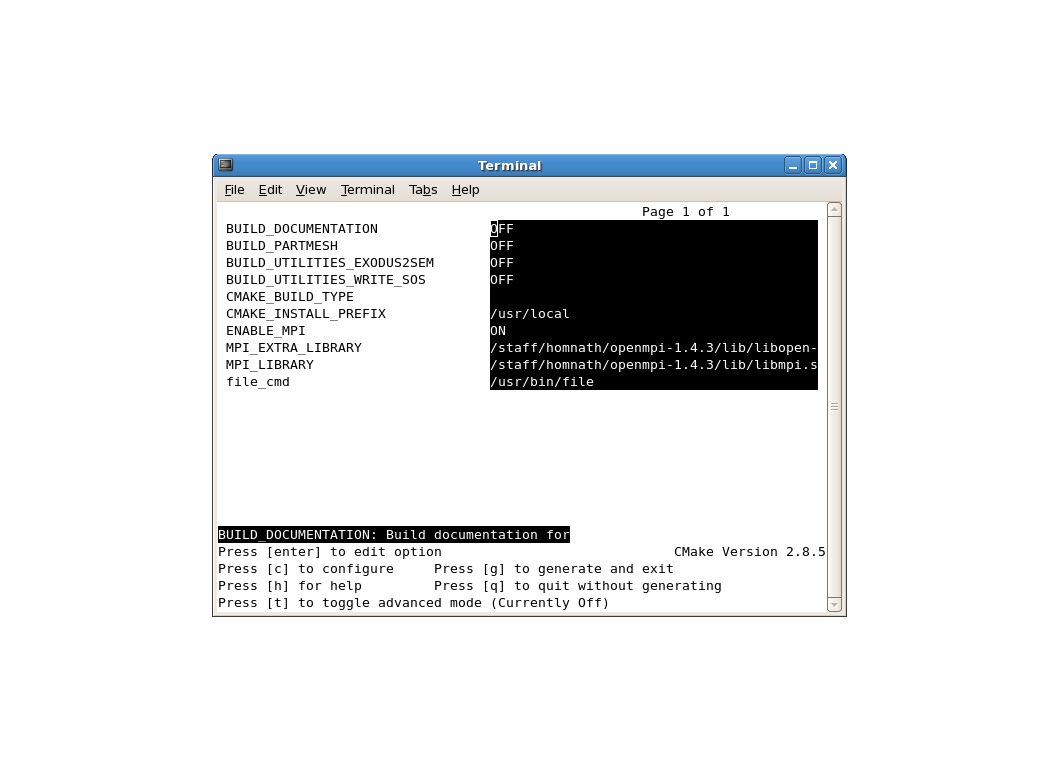
\includegraphics[scale=1.0]{cmake}
\caption{CMake configuration of \pack\ .}
\label{fig:cmake}
\end{figure}

CMake configuration is an iterative process (See Figure~\ref{fig:cmake}):
\begin{itemize}
\item Configure (c key or Configure button)
\item Change variables' values if necessary
\item Configure (c key or Configure button)
\end{itemize}

If WARNINGS or ERRORS occur, press the e key (or the OK button) to return to configuration. These steps have to be repeated until successful configuration. Then, press the g key (or the Generate button) to generate build files. Check carefully that all necessary variables are set properly. Unless configuration is successful, generate is not enabled. Sometimes, the c key (or Configure button) has to be pressed repeatedly until generate is enabled. Initially, all variables may not be visible. To see all variables, toggle advanced mode by pressing the t key (or the Advanced button).
To set or change a variable, move the cursor to the variable and press Enter key. If the variable is a boolean (ON/OFF), it will flip the value on pressing the Enter key. If the variable is a string or a file, it can be edited. For more details, please see the CMake documentation (\texttt{www.cmake.org}).
\\

Following are the main CMake variables for the \pack\ (See Figure~\ref{fig:cmake})

\colorbox{gray}{
\parbox{15.5cm}{
\begin{adescription}{BUILD\_UTILITIES\_EXODUS2SEM}
\item[BUILD\_DOCUMENTATION]           : If \texttt{ON}, the user manual (this file) is created. The default is \texttt{OFF}.
\item[BUILD\_PARTMESH]                : If \texttt{ON}, the \texttt{partmesh} program is built. The default is \texttt{OFF}. The \texttt{partmesh} program is necessary to partition the mesh for parallel processing.
\item[BUILD\_UTILITIES\_EXODUS2SEM]   : If \texttt{ON}, the \texttt{exodus2sem} program is built. The default is \texttt{OFF}. The \texttt{exodus2sem} program convert exodus mesh file to input files required by the \pack\ package (see also Chapter~\ref{chap:util}).
\item[BUILD\_UTILITIES\_WRITE\_SOS]   : If \texttt{ON}, the \texttt{write\_sos} program is built. The default is \texttt{OFF}. The \texttt{write\_sos} program writes a EnSight SOS file necessary for the parallel visualization (see also Chapter~\ref{chap:util}).
\item[ENABLE\_MPI]                    : If \texttt{ON}, the main parallel program \texttt{psemgeotech} is built otherwise main serial program \texttt{semgeotech} is built. The default is \texttt{OFF}.
\item[SCOTCH\_LIBRARY\_PATH]          : This is required if \texttt{BUILD\_PARTMESH} is \texttt{ON}. If not found automatically, it can be set manually.
\item[CMAKE\_Fortran\_COMPILER]       : This defines the Fortran compiler. If not found automatically or the automatically found compiler is not correct, it can be set manually.
\end{adescription}
}}\\

{\emph{Note 1: If}} \texttt{CMAKE\_Fortran\_COMPILER} {\emph{has to be changed, first change this and configure, and then change other variables if necessary and configure.}}\\
{\emph{Note 2: Even if some of the above variables are set }} \texttt{ON}{\emph{, if appropriate working compilers are not found, corresponding variables are internally set}} \texttt{OFF} {\emph{with WARNING messages.}}

\section{Compile}
\begin{itemize}[]
  \item Once configuration and generation are successful, the necessary build files are created. Now to build the main program, type: \\
  \texttt{make}

  \item On multi-processor systems (let's say eight processors), type:\\
  \texttt{make -j 8}

  \item To clean, type\\
  \texttt{make clean}
  \item{\emph{Note: If reconfiguration is necessary, it is better to delete all Cache files of the build directory.}}
\end{itemize}

\section{Run}
\subsubsection{Serial run}
\begin{itemize}[-]
\item To run the serial program, type \\
    \texttt{./bin/semgeotech} \emph{input\_file\_name}

    Example:

    \texttt{./bin/semgeotech ./input/validation1.sem}

\end{itemize}

\subsubsection{Parallel run}
\begin{itemize}[-]
\item To partition the mesh, type \\
    \texttt{./bin/partmesh} \emph{input\_file\_name}

    Example:

    \texttt{./bin/partmesh ./input/validation1.psem}

\item To run the parallel program, type \\
    \texttt{mpirun -n} \emph{number\_of\_nodes} \texttt{./bin/psemgeotech} \emph{input\_file\_name} \\

    OR

    \texttt{mpirun -n} \emph{number\_of\_nodes} \texttt{-{}-hostfile} \emph{host\_file} \texttt{./bin/psemgeotech} \emph{input\_file\_name}

    Example:

    \texttt{mpirun -n 8 ./bin/psemgeotech ./input/validation1.psem}
\end{itemize}

{\emph{Note: see Chapter~\ref{chap:input} for details on input and input files. Try to run one or more examples included in}} \texttt{input/}{\emph{. By default, example files included in the package are not copied to build directory during build process. If necessary, copy files within}} \texttt{input/} {\emph{folder of source directory to the}} \texttt{input/} {\emph{folder of build directory.}}

